%Background image credits:https://commons.wikimedia.org/wiki/File:CannabisBud.jpg Thomas Elliott, CC0, via Wikimedia Commons
\documentclass[a4paper, 11pt, oneside, polutonikogreek, english]{article}
\usepackage{lmodern}
\usepackage[T1]{fontenc}
% Load encoding definitions (after font package)
\usepackage[dvipsnames]{xcolor}
\usepackage{eso-pic,graphicx}
\usepackage[top=57mm, bottom=57mm, outer=33mm, inner=33mm]{geometry}
\setlength{\columnsep}{90pt}
\definecolor{customColor}{RGB}{221,229,194}
% Load encoding definitions (after font package)

% Load encoding definitions (after font package)

\usepackage{textalpha}

\usepackage{listings}
\lstset{basicstyle=\ttfamily}
\usepackage{pdflscape}

% Babel package:
\usepackage[english]{babel}
\usepackage{wasysym}

% With XeTeX$\$LuaTeX, load fontspec after babel to use Unicode
% fonts for Latin script and LGR for Greek:
\ifdefined\luatexversion \usepackage{fontspec}\fi
\ifdefined\XeTeXrevision \usepackage{fontspec}\fi

% ``Lipsiakos'' italic font `cbleipzig`:
\newcommand*{\lishape}{\fontencoding{LGR}\fontfamily{cmr}%
		       \fontshape{li}\selectfont}
\DeclareTextFontCommand{\textli}{\lishape}

\usepackage{booktabs}
\usepackage{graphicx}
\setlength{\emergencystretch}{15pt}
\graphicspath{ {./ } }
\usepackage[figurename=]{caption}
\usepackage{float}
\usepackage{fancyhdr}
\usepackage{microtype}

\usepackage{setspace}
\onehalfspacing

% change color of text, example replace all \color{Goldenrod} with \color{lightgray}

\makeatletter % change only the display of \thepage, but not \thepage itself:
\patchcmd{\ps@plain}{\thepage}{\color{customColor}{\thepage}}{}{}
\makeatother

\color{customColor}

\begin{document}
\AddToShipoutPictureBG{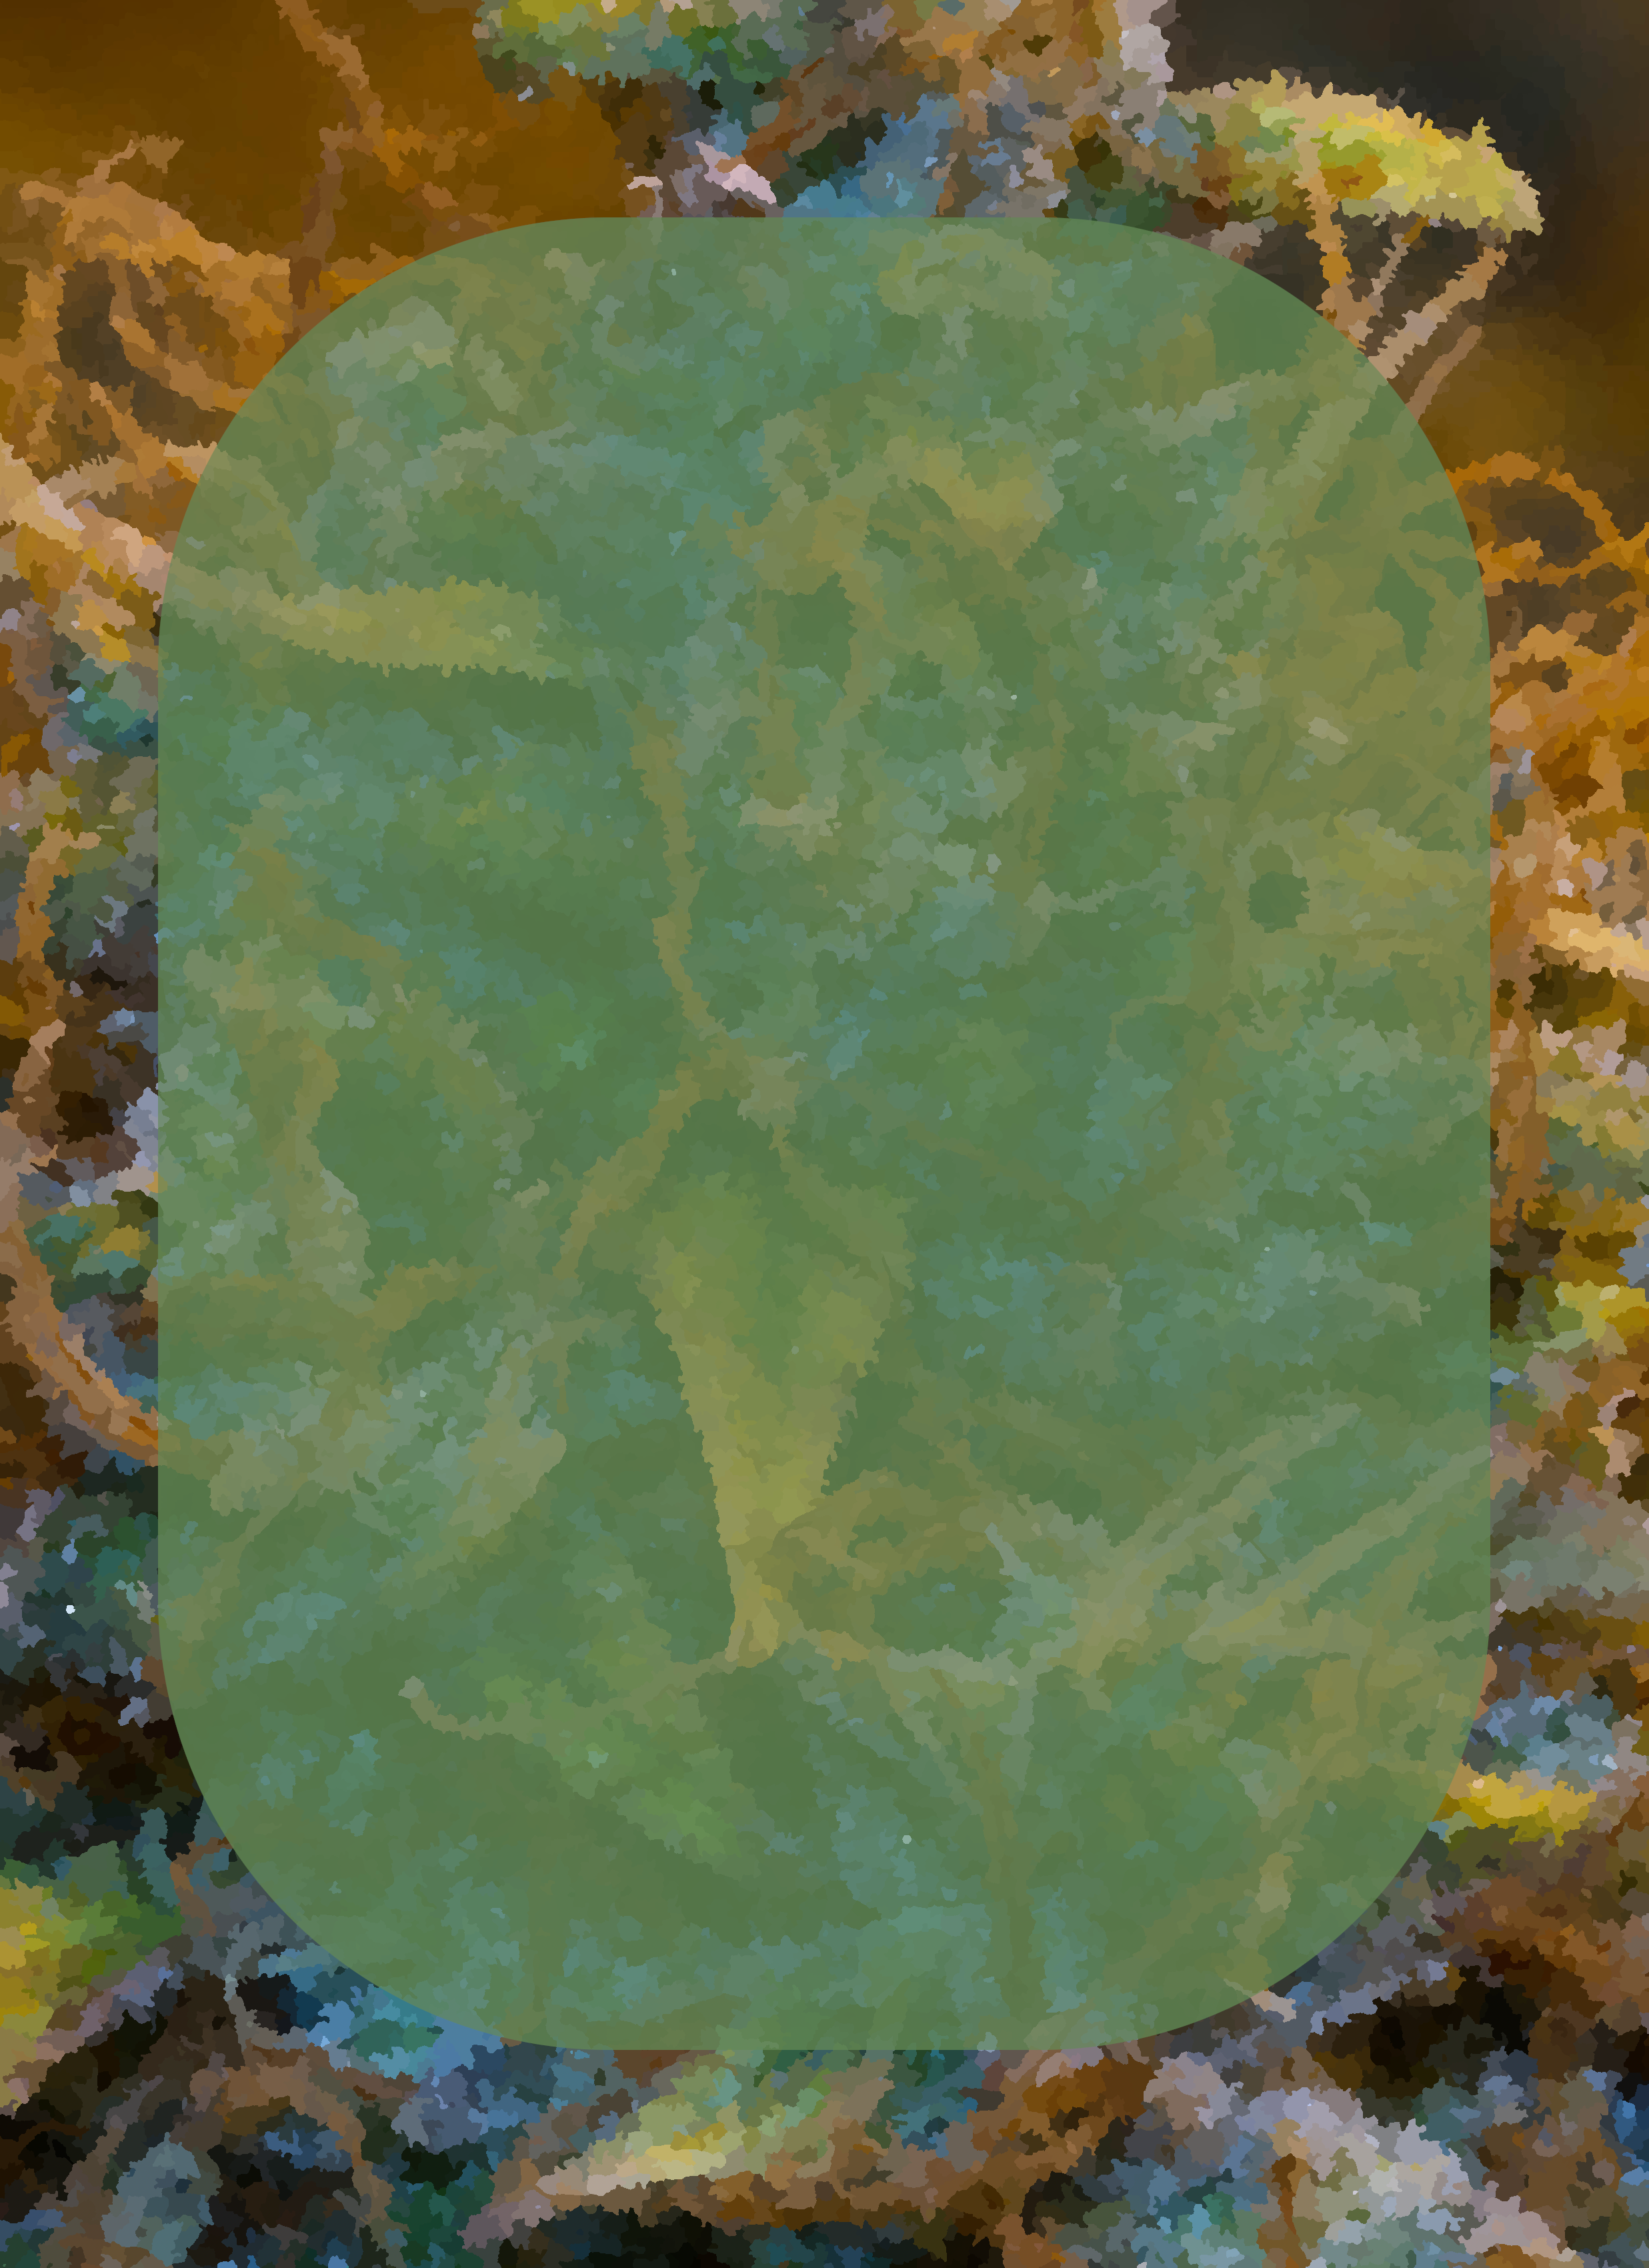
\includegraphics[width=\paperwidth,height=\paperheight]{CannabisBud.png}}
\begin{titlepage} % Suppresses headers and footers on the title page
	\centering % Centre everything on the title page
	%\scshape % Use small caps for all text on the title page

	%------------------------------------------------
	%	Title
	%------------------------------------------------
	
	\rule{\textwidth}{1.6pt}\vspace*{-\baselineskip}\vspace*{2pt} % Thick horizontal rule
	\rule{\textwidth}{0.4pt} % Thin horizontal rule
	
	\vspace{1\baselineskip} % Whitespace above the title
	
	{\scshape\Huge Specimen Inaugurale Medicum \\de Cannabis vi Medica}

	\vspace{1\baselineskip} % Whitespace above the title

	\rule{\textwidth}{0.4pt}\vspace*{-\baselineskip}\vspace{3.2pt} % Thin horizontal rule
	\rule{\textwidth}{1.6pt} % Thick horizontal rule
	
	\vspace{1\baselineskip} % Whitespace after the title block
	
	%------------------------------------------------
	%	Subtitle
	%------------------------------------------------
	
	{\scshape Quod Consensu Facultatis Medicae Halensis, ut Gradum Doctoris Medici a Dipisceretur, ad Diem 24. April 1803.} % Subtitle or further description
	
	\vspace*{1\baselineskip} % Whitespace under the subtitle
	
        {\scshape Eruditis ventilandum obtulit\\\Large Michaelis Jacobus Seidenschnur,\\\normalsize Hamburgensis.} % Subtitle or further description

	%------------------------------------------------
	%	Editor(s)
	%------------------------------------------------
        \vspace*{\fill}

	\vspace{1\baselineskip}

	{\small\scshape Halae, 1803.}
	
	{\small\scshape{In Officina Batheana}}
	
	\vspace{0.5\baselineskip} % Whitespace after the title block

        \scshape Internet Archive Online Edition% Publication year
	
	{\scshape\small Namensnennung Nicht-kommerziell Weitergabe unter gleichen Bedingungen 4.0 International} % Publisher
\end{titlepage}
\setlength{\parskip}{1mm plus1mm minus1mm}
\clearpage
\section{}
\paragraph{}
Domeyerus nuper in diario πολυθρυλλήτῳ, quod Hufelandius, Schregerus et Harlesius edunt,\footnote{Journal der ausländ. medic. Literatur, J. 1802. S. 74-76.} remedium quoddam Mauricum, Haschisch nomine, tanquam novum priusque inauditum ut et praestantissimum praedicavit, cum opio palmam eripere ipsi videretur. Quaecunque Londinensis ille medicus de efficacia ejus remedii praecepit, mira videbantur atque praeclara cuivis lectori; namque et hilaritatem gignere et insomnia laeta et somnum placidissimum, et corpus recreare, sine ulla noxa, et stomachum firmare fame aucta, nec caput tentare nec nauseam ciere nec alvum stipare ferebatur. Drachmam autem sumi a Mauris foliorum in pulverem redactorum, ipsaque folia, loco foliorum Nicotianae fumo sugi. Mirum eum pulverem missum esse clarissimo Banksio ex Africa, haberi autem a variis pro foliis cannabis sativae in pulverem redactis, licet Mauri negent ipsam eam plantam esse, e qua funes parentur. Hae sunt, quae Domeyerus de novo illo remedio narrat.
\section{}
\paragraph{}
Statim vero cuivis, qui vel Russelii celeberrimum librum legerit,\footnote{Naturgeschichte von Aleppo, B. 1. S. 165.} in mentem veniet, tantum abesse ut novum sit id remedium, ut potius ab omni inde antiquitate per totum orientem adhibitum fuerit nomine Haschisch vel ad hilaritatem suaviaque deliria promovenda vel ad somnum placidum ciendum.

Namque Russelius refert, nomine Haschisch arabico, et Binusch indico comprehendi pulverem cannabis feminae foliorum, chartae humidae involutum, cineribus calidis immersum, donec pasta inde fiat, quam in morsulos concisam siccent populi orientales. Ejus pulveris grana pauca, cum dulcibus, maxime cum ficubus mixta, inebriare ac obstupefacere: drachmam dimidiam vero, cum foliis Nicotianae fumo suctam simili modo ebrios reddere ac deliria producere.

Confirmat ea saeculi decimi sexti peregrinator celeberrimus, Prosper Alpinus.\footnote{De medic. Aegypt. f. 121. b. (Paris 1645. 4).} „Assis (Haschisch) nil aliud est, quam pulvis e cannabis foliis paratus, quem cum aqua dulci mistum in massam redigunt, cujus bolos quinque castaneae magnitudinis, vel plures devorant, a quibus per horam post homines, qui eam sumsere, quasi ebrii facti, suas amentias produnt, atque in ecstasi diu manentes, suis desideratis visionibus oblectantur, hocque medicamenti genus plebs frequentat quia viliori pretio ibi venditur. Qua mira ejus facultate ista herba apud ipsos, ut jam dictum est, nomen assis adsecuta est, quod per excellentiam herbam dicit.“\footnote{Solo discrimine eo id verum est, quod Haschischa herbam, Haschisch vero vel succum vel pulverem cannabis denotet.} Similia narrant Hasselquistius\footnote{Resa til heliga landet, p. 512.} et Niebuhrius.\footnote{Beschreibung von Arabien, S. 57.}
\section{}
\paragraph{}
Uberius et disertius hanc substantiam in oriente tantopere depraedicatam illustravit Engelb. Kämpferus, qui exeunte saeculo decimo septimo Persiam peragravit. Cannabin eam, quae inebrians remedium illud praebet, ut ovum ovo, in omnibus nostrati similem habet, neque varietatem levissimam, quam Indi Bangue appellant,\footnote{Rheed. hort. Malab. tom. 10. p. 119.} tanquam speciem esse considerandam. Virtutem vero suam non in quovis solo et sub quolibet caelo adipisci, namque solummodo in agro urbis Ispahan et in Luristana et apud Caseruna genuinam alere suam efficaciam. „Semen inquit,\footnote{Amoenit. exot. p. 645. seq.} virtutem obtinet debiliorem; incoquitur cibis, et ingreditur emulsiones, ordinandas ad laetitiae crapulam inducendam. Alii semen saccharo saleve condunt, vescendum ad gaudia etiam conjugibus inducenda. Pultes, dum Cracoviae studerem, ex farina seminis cannabini per jejunia saepe comedimus, ex quibus vero crapulosum me vel in gaudia effusum esse non memini.“ E polline quoque florum, per linteum cribrato, parari probatissimam earum gentium substantiam, dum in trochiscos redigatur; tres esse fere ejus species; primam ac praestantissimam, cujus trochisci fracti scinillis micent, interno usui commendatam; alteram viliorem, sputo humano mixtam, tabaco jungi; tertiam iidem usui dicatam. Praeterea describit modum parandi Haschisch, quem a Derwischi persicis didicerit: Folia cannabis aqua adfusa adsiduo agitabant, dein aquam, expressis leniter foliis, abiiciebant; adfusa aqua recenti alia, quam cum pulvere aliquoties agitatam, denuo abiiciebant. Pulverem gemina vice elutum expressumque subiiciebant pistillo obeso ligneo, et in vase fictili non incrustato acerrime terebant, donec redactus esset in pultem. Huic paullatim adfundebant aquam recentem, rotabant continuo, et demum per linteum trajiciebant, omni, praeter recrementa, permeante substantia: ex qua ipse colatus liquor virescebat. E liquore, is qui praeparaverat, scyphum, dimidiae librae capacem, singulis admetiebatur sociis, affatim evacuandum, rotato subinde vase ne farina subsideret. Hoc liquore, velut mero, delibuti et ad laetitiam conformati, se reddebant itineri. Sunt, qui pulverem cum syrupo subigunt, pro efformandis placentis et bolis, in eumdum usum deglutiendis. A foliis cannabinis, velut a potiori inebriantium specie, homines ebriosi in Persia Indiaque vulgo appellantur Bengi.

Per totam Persiam in tabernio praesto esse liquorem ex infusis aqua foliis, quo mire recreentur viatores, testatur ἀυτόπτης Chardinus.\footnote{Voyage en Perse, tom. 4. p. 207.} In India homines a nimio cannabis usu furibundos evadere, pugnaces; nonnunquam continuo plorare, interdum jugiter ridere, narrat Rumphius.\footnote{Herbar. Amboin. tom. 5. p. 210.} Quin in ipsa Africa australi cannabis insignem copiam coli, cujus foliis utantur Hottentotti et Caffri ut sese inebrient, referunt Sparrmannus\footnote{Resa til goda Hopps udden, p. 468.} et Thunbergius.\footnote{Resa uti Europa etc. D. I. p. 212.}
\section{}
\paragraph{}
Ex India in Tatariam orientalem migrasse videtur usus cannabis. Refert enim Falkius,\footnote{Beiträge zur topograph. Kenntn. des russischen Reichs, B. 2. S. 265.} Bukharos fasciculis floram cannabinorum impraegnare aquam, bolos quoque hilaritatis conficere ex hisce fasciculis, dum eos intra folia brassicae in cineribus calidis insudare sinant et haec cremore lactis tincta assataque in bolos redigant.

Condimenta varia in Malabaria fieri e foliis cannabis cum moscho, ambra, camfora, areca, et caryophyllis, referant Garcias ab Orto\footnote{Clus. exot. p. 258.} et Christoph. a Costa.\footnote{Ib. p. 290.}

Ipsa semina cannabis a Persis tanquam aphrodisiacum considerari, a quo tamen sterilitas efficiatur, Olearius narrat.\footnote{Orient. Reiser S. 529.}
\section{}
\paragraph{}
His expositis patet, quantopere celebratum sit Haschisch per totum orientem. Exspatiari autem in antiquitates liceat, ut, quantopere novitas hujus remedii veritati repugnet, luculenter prodeat. Primus fere, qui cannabis vires medicas praedicat, est Plinius.\footnote{Hist. natur. lib. 20. c. 23.} Is semine cannabis genituram virorum exstingui; succum vero ex eo vermiculos aurium et quodcunque animal intraverit, necare, sed cum dolore capitis, perhibet. Tantam autem vim ejus esse, ut aquae infusus coagulare eam dicatur. Radicem in aqua coctam articulos contractos resolvere, item podagras et similes impetus. Ambustis crudam illiniri, sed saepius mutari prius quam arescat. Dioscorides confirmat, quae Plinius de sterilitate semine producta narrat.\footnote{Lib. 3. c. 165. p. 240. ed. Sarrac.} Distinguit autem sylvestrem a sativa cannabi, illam resolvere, dum cataplasmate illinatur, oedemata et phlegmones et callos. Galenus eadem fere habet de seminis virilis diminutione et usu contra otalgias.\footnote{De facult. simpl. lib. 7. p. 87. ed. Basil. graec.} Alio loco vero refert, cum τραγήμασι, (cupediis) mixtam cannabin δυστπέπτην esse et κακοστόμαχον et κεφαλαλγέα et κακόχυμον et θερμαίνοντα. Repetunt haec fere Aëtius\footnote{Tetr. l. serm. 1. col. 29. ed. Stephan.} et Paullus Aegineta.\footnote{Lib. 7. p. 239. ed. Basil. graec.}

Repetunt etiam Arabes, sed sedulo distinguunt Kannab, plantam ipsam, a Schehedanedsch, seminibus, et ab Haschisch, seu succo narcotico. Sic Serapion sub nomine Schehedanedsch virtutes cannabis e Graecis exscribit\footnote{Simpl. c. 207. f. 153. b.}: sic Mesue sub nomine Kannab.\footnote{Rhac. contin. lib. 22. c. 461. f. 448. d.} Avicenna identidem.\footnote{Can. lib. 2. p. 248. 256. ed. arab. Rom.} Alio loco vero, de Haschisch loquens, fortius esse remedium ipso euphorbio,\footnote{Posset tamen etiam pro Euphorbio, mutatis literis arabicis, legi Opium.} adfirmat, interficere super drachmam potum, adurere stomachum et vomitum ciere.\footnote{Ib. p. 178.}
\section{}
\paragraph{}
His omnibus rationis trutina pensitatis, patet:
\begin{itemize}
    \item[a.] Haschisch illud remedium novantiquum esse, atque ab Arabum medicorum inde temporibus praedicatum.

    \item[b.] Cannabin vere sativam esse, e qua, vario modo, parant orientales populi pharmaca et inebriantia et exhilarantia. Etenim nullum, etiam sagacissimis botanicis, sese obtulit discrimen specificum inter orientalem et nostratem cannabin.

    \item[c.] Nostratem cannabin narcotica virtute variarum suarum partium gaudere, vel inde elucet, quod Lindestolpius\footnote{De venenis, p. 541.} adserit, ex diuturniore mora vel somno capto in agris, quibus cannabis sata reperitur, visum debilitari, imo vertiginem et ebrietatem consequi.

    \item[d.] Varietatem tamen singularem eligi in oriente ad conficiendas cupedias Muhammedanorum, quae Haschisch dicuntur, cum ipse Kämpferus (l. c.) contendat, non quovis solo easdem exserere virtutes, sed praestantiorem ceteris esse, quae circa Ispahanum crescat. Eam soli efficaciam et culturae etiam in nostratibus plantis culinaribus saepenumero animadvertimus. Brassica Rapa, unica species, infinitas pro soli varietate ostendit vicissitudines, quorsum marchicae praesertim rapae pertinent, in quovis alio, extra Marchiam, solo degenerantes. Scimus etiam Papaver somniferum, unicam speciem, in oriente Opium exhibere, a succo capitum nostratis papaveris diversum. Rheum undulatum et palmatum radices in Germania fert haudquaquam iis virtutibus praeditas, quas in tatarico et mongolico Rhabarbaro observamus.

    \item[e.] Contraria sibi sunt, quae veteres et recentiores de dosi Haschisch proferunt. Avicenna enim, interfici, qui drachma plus sumserit; Domeyerus et ante eum Prosper Alpinus drachmam unam quavis vice propinari adserunt. Oppositas sibi eas relationes ita conjungi posse existimo, si variorum parandi modorum rationem habuerimus. Kämpferus enim et Prosper Alpinus et Russelius, modo cum opio, jam cum aromatibus, nunc cum saccharo solo aut aliis τραγήματι misceri referunt, a quibus virtus hujus remedii et efficacia mire mutari debet.
\end{itemize}
\section{}
\paragraph{}
Quod superest, addenda quaedam sunt de vi medica, quam semina cannabis adversus icterum exercere dicuntur. A pluribus inde saeculis per Belgium celebratum est euporiston e cannabis seminibus paratum, quae cum aqua trita emulsionem praebent.\footnote{Dodon. pempt. 4. lib. 2. c. 26. p. 535.} Modum, quo semina cannabis quandoque utiliter agere possunt in hoc morbo, divinare possumus ex observatione Sylvii, qui solis cum lacte coctis seminibus cannabis plures semet curasse ictericos et a plebeiis vidisse curatos narrat. Coquitur ad eum finem manipulus unus seminum cannabis in mensura lactis bubuli, donec semina rupta fuerint, colatum decoctum bis terve de die ad uncias quinque aut sex sumitur.\footnote{Sylv. prax. med. lib. 1. p. 302. 306.} E celeriori effectu patet, narcotica sua virtute egisse haec semina contra spasmum, verosimilem icteri hujus caussam. Ita etiam Herlizius refert\footnote{Murray appar. medic. vol. 4. p. 619.} in ictero epidemico Goettingensi promtissime juvasse semina cannabis eo modo cocta.
\section{}
\paragraph{}
Denique ad externum usum oleum blandum seminum cannabis commendatur, iisdem certe viribus praeditum ac papaveris oleum. Hinc iniicitur in urethram, dum blennorrhoea laborat: solent etiam in hoc morbo theae forme infusum cannabis seminum commendare, ut ardor doloresque mitigentur, in quo congruunt Todius\footnote{Kenntn. und Heilung des gem. Trippers, S. 271. 309.} et Murrayus.\footnote{Opuse. vol. 2. p. 443. 446.}
\clearpage
\end{document}
